% compile with: pdflatex -shell-escape filename.tex
\documentclass[crop,tikz,convert=pdf2svg]{standalone}
\usetikzlibrary{automata}

\tikzset{
  ->,
  >=latex,
  every state/.style={thick, fill=gray!10},
  initial text=$ $,
  node distance=3cm,
}

\begin{document}

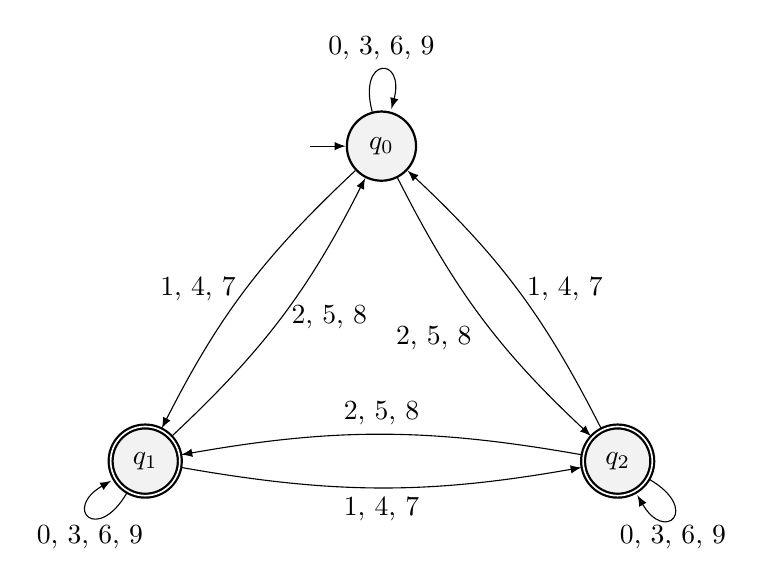
\begin{tikzpicture}
  \node[state, initial] (q0) at (0, 0) {$q_0$};
  \node[state, accepting] (q1) at (-3, -4) {$q_1$};
  \node[state, accepting] (q2) at (3, -4) {$q_2$};
  \draw
  (q0) edge[loop above] node{0, 3, 6, 9} (q0)
  (q0) edge[bend right=10,left] node{1, 4, 7} (q1)
  (q0) edge[bend right=10,below left] node{2, 5, 8} (q2)
  (q1) edge[bend right=10,right] node{2, 5, 8} (q0)
  (q1) edge[in=210,out=240,loop,below] node{0, 3, 6, 9} (q1)
  (q1) edge[bend right=10,below] node{1, 4, 7} (q2)
  (q2) edge[bend right=10,right] node{1, 4, 7} (q0)
  (q2) edge[bend right=10,above] node{2, 5, 8} (q1)
  (q2) edge[in=300,out=330,loop,below] node{0, 3, 6, 9} (q2)
  ;
\end{tikzpicture}

\end{document}
